\section{离散近似与过程极限（进阶）}
\label{sec:ctsp-process-limits}

本章多次借用一个直觉：步长很小的随机游走“看起来像”Brownian运动，微小增量的Markov链“看起来像”扩散。第~\ref{sec:ctsp-brownian}节用它引出$\sqrt{\Delta t}$缩放，第~\ref{sec:ctsp-numerical}节用它构造数值格式。本节说明这个直觉在什么意义下成立：不仅每个固定时刻的分布收敛，整条随机路径的分布也收敛。这比逐时刻的极限多了对整条路径的控制，因而需要额外的条件。本节是进阶内容，前两节的采样与随机逼近结论并不依赖这里的路径极限理论。

\subsection{路径距离与紧性}
\label{sec:ctsp-path-space}

\paragraph{连续路径的一致距离}
要说一列随机路径的分布收敛，先要规定两条路径怎样才算接近。对$[0,T]$上的连续实值路径，自然的距离是一致距离$\|x-y\|_\infty=\sup_{t\leq T}|x(t)-y(t)|$。连续路径空间$C([0,T])$在这一距离下完备可分，是Polish空间，因而可以使用分布弱收敛的一般理论。随机路径$X_n$的分布弱收敛到$X$，记作$X_n\Rightarrow X$，指对$C([0,T])$上每个有界连续泛函$F$，$\mathbb EF(X_n)\to\mathbb EF(X)$。

这里有两种不同的“接近”。若$X_n$与$X$定义在同一概率空间上，可以问$\|X_n-X\|_\infty$是否依概率趋零，这是第~\ref{sec:ctsp-error-types}节强误差的路径版本，需要把两者耦合起来。分布弱收敛则不要求耦合，只比较路径的规律；它是弱误差的路径版本，随机游走与Brownian运动通常生活在不同的概率空间上，能谈论的只有这一种。

\paragraph{跳跃路径与Skorokhod时间对齐}
跳跃路径不能用一致距离比较。设$x(t)=\mathbb I\{t\geq\frac12\}$，$x_n(t)=\mathbb I\{t\geq\tau_n\}$，$\tau_n\downarrow\frac12$。两条路径只是跳跃时刻略有错开，直觉上应当很接近；但在两次跳跃之间，一条已经取$1$，另一条仍取$0$，所以$\|x_n-x\|_\infty=1$对所有$n$成立。图~\ref{fig:ctsp-path-space-examples}(a)画出了这一情形。

\term{Skorokhod拓扑}（Skorokhod $J_1$ topology）允许先把时间轴轻微地拉伸或压缩，再比较取值。若存在严格递增的连续双射$\lambda_n:[0,T]\to[0,T]$，使
\[
  \|\lambda_n-\mathrm{id}\|_\infty\to0,\qquad\|x_n\circ\lambda_n-x\|_\infty\to0 ,
\]
就称$x_n$在$J_1$意义下收敛到$x$。在上面的例子中，取经过$(0,0)$、$(\frac12,\tau_n)$、$(1,1)$的分段线性$\lambda_n$，它把$x$的跳跃时刻送到$x_n$的跳跃时刻，于是$x_n\circ\lambda_n=x$，而$\|\lambda_n-\mathrm{id}\|_\infty=\tau_n-\frac12\to0$。右连续有左极限的路径空间$D([0,T])$在这一拓扑下也可以赋予完备可分的度量\scite{math-kallenberg2021probability}。若极限路径连续，$J_1$收敛与一致收敛等价。

\paragraph{有限维收敛的不足}
最直接的猜想是：只要每组有限个时刻上的联合分布收敛，路径分布就收敛。下面的确定性例子说明这不够。令
\[
  x_n(t)=\max\{1-n^2|t-1/n|,0\},\qquad t\in[0,1],\ n\geq2 ,
\]
它是一个以$1/n$为中心、高为$1$、宽为$2/n^2$的尖峰，见图~\ref{fig:ctsp-path-space-examples}(b)。固定任意时刻$t$，当$n$足够大时尖峰已经移到$t$的左侧并且宽度小于$t$，所以$x_n(t)\to0$；任意有限个时刻同时如此。可是$\|x_n\|_\infty=1$，$x_n$在$C([0,1])$中不收敛到零。越来越窄的尖峰从有限个截面之间溜过，有限维分布看不到它。

\begin{figure}[htbp]
  \centering
  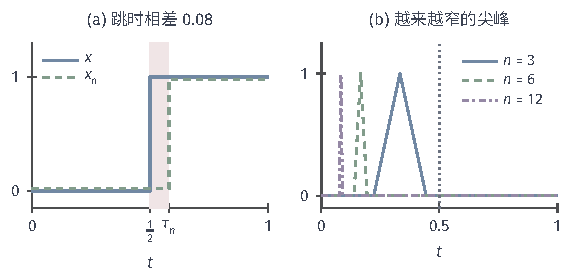
\includegraphics[width=97mm]{figures/03-optimization-evolution-and-signals/02-processes-and-trajectory-evolution/tikz/ctsp-path-space-examples/figure.pdf}
  \caption{路径空间中的两种比较（解析式教学图）。(a)跳跃时刻分别为$\frac12$与$\tau_n=0.58$的两条阶梯路径（绿线略向内偏移以便辨认），浅红带内二者相差$1$，一致距离为$1$，经时间对齐后的$J_1$距离不超过$0.08$；(b)尖峰$x_n(t)=\max\{1-n^2|t-1/n|,0\}$，$n=3,6,12$。任一固定时刻（如点线$t=\frac12$）最终只看到零，路径的最大值却始终为$1$。}
  \label{fig:ctsp-path-space-examples}
\end{figure}

\paragraph{紧性判据}
缺的是对路径整体形状的统一控制。对连续路径，这由Arzelà--Ascoli定理刻画：$C([0,T])$中的一族函数相对紧，当且仅当它们在起点处一致有界并且等度连续，即对每个误差阈值，能选同一个时间间隔同时控制族内所有函数的短时变化。把这一判据翻译成概率语言，用连续模
\[
  w(x,\delta)=\sup\{|x(t)-x(s)|:s,t\in[0,T],\ |t-s|\leq\delta\}
\]
描述短时振荡，就得到路径分布紧性的判据。

\begin{theorem}[连续路径的紧性]
  \label{thm:ctsp-tightness}
  设$X_n$是$C([0,T])$值的随机路径。若$(X_n(0))_n$的分布一致紧，并且对每个$\varepsilon>0$，
  \[
    \lim_{\delta\downarrow0}\sup_n\mathbb P\bigl(w(X_n,\delta)>\varepsilon\bigr)=0 ,
  \]
  则$(X_n)$的分布族一致紧。
\end{theorem}

\begin{proof}
固定$\eta\in(0,1)$。选$M$使$\sup_n\mathbb P(|X_n(0)|>M)\leq\eta/2$；对$k=1,2,\ldots$，选$\delta_k\downarrow0$使$\sup_n\mathbb P(w(X_n,\delta_k)>2^{-k})\leq\eta2^{-k-1}$。由联合界，每个$X_n$以至少$1-\eta$的概率落入集合$\mathcal K=\{x:|x(0)|\leq M,\ w(x,\delta_k)\leq2^{-k}\ \forall k\}$。$\mathcal K$中的函数等度连续；把$[0,T]$分成长度不超过$\delta_1$的有限段，又得到统一的幅度界。由Arzelà--Ascoli定理，$\mathcal K$的闭包是紧集。
\end{proof}

Arzelà--Ascoli定理可参考文献\scite{math-folland1999real}。

增量矩界是检验振荡条件的常用充分条件：若存在$p,\beta,C>0$，使对所有$n$与$s,t$，$\mathbb E|X_n(t)-X_n(s)|^p\leq C|t-s|^{1+\beta}$，并且初值一致紧，则振荡条件成立。这是第~\ref{chap:stochastic-processes-and-sample-paths}章Kolmogorov连续性准则的一致版本：常数对整列过程统一。

跳跃路径不能使用连续模：一次合法的跳跃就使$w(x,\delta)$无法随$\delta$趋零。$D([0,T])$中的紧性要换用其他判据，常用的是Aldous条件：路径在有界时间内以高概率停留在紧集中，并且对任意有界停时$\rho_n$与趋于零的常数$\delta_n$，$X_n(\rho_n+\delta_n)-X_n(\rho_n)\to0$依概率成立\scite{math-kallenberg2021probability}。它要求的是“在随机时刻之后的短时间内不发生大的变化”，允许跳跃但排除跳跃的聚集。两种判据针对不同的路径空间，不能混用。

\subsection{从有限维分布识别过程极限}
\label{sec:ctsp-identify-limit}

\paragraph{子列极限与识别}
紧性本身不给出极限，只保证极限点存在。证明过程收敛的标准路线分两步。第一步，由紧性与Prokhorov定理，路径分布的每个子列都有进一步的子列弱收敛；Prokhorov定理与弱收敛的一般性质见\BookChapterRef{chap:weak-convergence-limit-theorems}{卷二“弱收敛与极限定理”章}。第二步，识别这些子列极限：若有限维分布收敛到某个过程$X$的有限维分布，则每个子列极限都与$X$有相同的有限维分布。

第二步之所以可行，是因为坐标映射$x\mapsto(x(t_1),\ldots,x(t_k))$在$C([0,T])$上连续，连续映射保持弱收敛，所以子列极限的有限维分布就是有限维分布的极限；而连续路径的分布由有限维分布唯一确定（路径空间的Borel $\sigma$代数由坐标映射生成）。于是所有子列极限相同，整列收敛：
\[
  \text{紧性}+\text{有限维分布收敛}\ \Longrightarrow\ X_n\Rightarrow X\quad\text{于}C([0,T]).
\]
在$D([0,T])$中，坐标映射只在路径连续的时刻连续，所以有限维收敛只需在极限过程几乎必然不跳的时刻核对；这样的时刻在$[0,T]$中稠密，足以确定分布。

\paragraph{连续映射与路径泛函}
过程收敛的用处在于把极限传递给路径泛函。若$X_n\Rightarrow X$于$C([0,T])$，$F$是在$X$的几乎每条路径处连续的泛函，则$F(X_n)\Rightarrow F(X)$。常见的泛函需要逐个核对连续性。
\begin{itemize}
  \item 最大值$F(x)=\max_{t\leq T}x(t)$与时间积分$F(x)=\int_0^Tg(x(t))\,\mathrm dt$（$g$连续有界）在一致距离下连续，可以直接传递。
  \item 首次到达时刻$\tau_a(x)=\inf\{t:x(t)\geq a\}$不是处处连续的。设$x$在$[0,1]$上从$0$线性升到$a$，在$[1,2]$上停在$a$，之后线性上升越过$a$；则$\tau_a(x)=1$，而$x-\frac1n$直到$t=2+\frac1n$才到达$a$，所以$\tau_a(x-\frac1n)\to2\neq1$。问题出在路径“碰到$a$却没有越过”。Brownian路径到达$a$后立即越过$a$（由强Markov性质与反射原理），这种接触几乎必然不发生，所以$\tau_a$在Brownian运动的几乎每条路径处连续，可以传递。
\end{itemize}
在$D([0,T])$中，最大值仍然连续，固定时刻的取值则只在极限路径于该时刻连续时连续。

\subsection{随机游走与扩散近似}
\label{sec:ctsp-donsker}

\paragraph{Donsker定理}
现在可以准确陈述第~\ref{sec:ctsp-brownian}节的直觉。设$\xi_1,\xi_2,\ldots$独立同分布，均值为零，方差为一，$S_k=\xi_1+\cdots+\xi_k$。对每个$n$，在时刻$k/n$放置值$S_k/\sqrt n$，并在相邻时刻之间线性插值，得到$C([0,1])$中的随机折线$X_n$。

\begin{theorem}[Donsker定理]
  \label{thm:ctsp-donsker}
  在上述条件下，$X_n\Rightarrow W$于$C([0,1])$，其中$W$是标准Brownian运动。
\end{theorem}

定理~\ref{thm:ctsp-donsker}称为\term{Donsker定理}（Donsker theorem），也称函数型中心极限定理。证明沿上一小节的两步进行\scite{math-kallenberg2021probability}。有限维分布的收敛来自多元中心极限定理：对$0<t_1<\cdots<t_k$，各段增量$S_{\lfloor nt_i\rfloor}-S_{\lfloor nt_{i-1}\rfloor}$相互独立，标准化后分别趋于$\mathcal N(0,t_i-t_{i-1})$，插值的修正项依概率趋零。紧性需要控制振荡；若再假设$\mathbb E\xi_1^4<\infty$，网格点上$\mathbb E(S_k-S_j)^4\leq C(k-j)^2$，于是$\mathbb E|X_n(t)-X_n(s)|^4\leq C'|t-s|^2$，上一小节的矩判据适用（网格间的插值段需要单独但简单的估计）。只有二阶矩时，紧性需要更精细的最大不等式。图~\ref{fig:ctsp-donsker}画出了同一列$\pm1$步长在三个尺度上的缩放折线：步数增加时，折线的锯齿变细，整体的起伏幅度保持在同一量级，逐渐呈现Brownian路径的样子。

\begin{figure}[htbp]
  \centering
  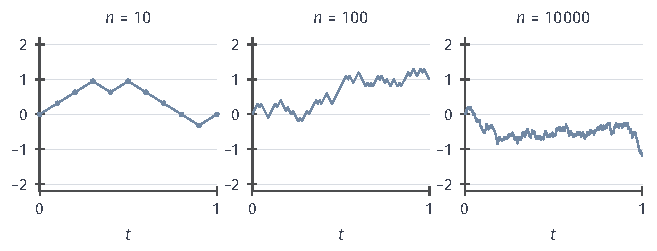
\includegraphics[width=111mm]{figures/03-optimization-evolution-and-signals/02-processes-and-trajectory-evolution/tikz/ctsp-donsker/figure.pdf}
  \caption{Donsker缩放。用同一列$10000$个独立等可能的$\pm1$步长（固定随机种子），分别取前$n=10,100,10000$步，画出$k/n\mapsto S_k/\sqrt n$的线性插值。纵向按$\sqrt n$、横向按$n$缩放后，三条折线的起伏幅度相当；$n$增大时局部锯齿变细，路径规律趋于Brownian运动。}
  \label{fig:ctsp-donsker}
\end{figure}

过程收敛加上连续映射，给出了离散问题的近似答案。例如
\[
  \max_{k\leq n}S_k/\sqrt n=\max_tX_n(t)\Rightarrow\max_{t\leq1}W_t ,
\]
由反射原理~\eqref{eq:ctsp-reflection}，
\[
  \mathbb P\Bigl(\max_{k\leq n}S_k\geq a\sqrt n\Bigr)\to2\bigl[1-\Phi(a)\bigr],\qquad a>0 .
\]
单时刻的中心极限定理只给出$S_n/\sqrt n$的分布，无法回答关于最大值的问题；这里需要的正是整条路径的收敛。

\paragraph{一般微小增量的扩散近似}
Donsker定理的增量独立同分布、条件均值为零。更一般的Markov链每一步的增量可以依赖当前状态，并且有小的漂移。设对每个$n$，$(X^n_k)_k$是Markov链，记增量$\Delta^n_k=X^n_{k+1}-X^n_k$，并在时间尺度$t=k/n$上观察。若在每个紧集上一致地有
\[
  \begin{aligned}
    n\,\mathbb E[\Delta^n_k\mid X^n_k=x]&\to b(x),\\
    n\,\mathbb E[(\Delta^n_k)^2\mid X^n_k=x]&\to a(x),\\
    n\,\mathbb E[|\Delta^n_k|^{2+\delta}\mid X^n_k=x]&\to0
  \end{aligned}
\]
（最后一条是Lindeberg型条件，排除单步的大跳跃），初值收敛，路径在有界时间内以高概率停留在紧集中，并且以$b$为漂移、$a$为扩散系数的鞅问题适定，那么$X^n_{\lfloor nt\rfloor}$收敛到相应的扩散\scite{math-kallenberg2021probability}。这类结论统称\term{扩散近似}（diffusion approximation）。漂移与扩散系数分别来自条件均值与条件二阶矩，乘以$n$是因为每单位时间有$n$步。

\begin{example}[Wright--Fisher扩散]
  \label{ex:ctsp-wright-fisher}
  规模为$n$的群体中某个等位基因的频率为$p$，下一代的$n$个个体独立地以概率$p$携带该基因，于是下一代频率是$\operatorname{Binomial}(n,p)/n$。增量的条件均值为$0$，条件方差为$p(1-p)/n$，四阶矩为$O(n^{-2})$。以$n$代为一个时间单位，条件均值与方差乘以$n$后分别为$0$与$p(1-p)$。频率过程收敛到扩散$\mathrm dX=\sqrt{X(1-X)}\,\mathrm dW$。它在$0$与$1$处噪声消失，这两个点是吸收态，与第~\ref{sec:ctsp-invariant}节讨论的不变分布不唯一的例子同类：基因最终要么消失，要么固定。
\end{example}

\paragraph{与平均ODE的对照}
扩散近似与第~\ref{chap:discrete-time-stochastic-processes}章随机逼近的平均ODE都描述“步长很小的随机递推”，但它们看的是不同的尺度，结论不能互换。以常步长$a$的递推$\theta_{k+1}=\theta_k+a[h(\theta_k)+\xi_{k+1}]$为例，$\xi$为条件方差$\sigma^2$的鞅差。在算法时间$t=ka$上观察，每单位时间有$1/a$步，条件均值乘以$1/a$得$h$，条件方差乘以$1/a$得$a\sigma^2\to0$。所以$a\to0$时，路径收敛到平均ODE $\dot\theta=h(\theta)$：噪声在这个尺度下消失。

若把偏离ODE轨迹的部分按$\sqrt a$放大，即考虑$(\theta_{\lfloor t/a\rfloor}-\bar\theta(t))/\sqrt a$，其中$\bar\theta$是ODE的解，噪声就重新以有限的强度出现，在适当条件下这一放大的偏差收敛到一个线性扩散（ODE附近的OU型过程）。前者回答“递推平均地往哪里走”，后者回答“围绕平均路径的波动有多大”。第~\ref{sec:ctsp-sa-lyapunov}节常增益情形的稳态方差$a\sigma^2/2$正是这种$\sqrt a$量级的波动。只改变记号而不改变尺度，就会把一种极限的结论误用到另一种上。
